\begingroup
\definecolor{loopsideroute}{RGB}{28,79,114}
\definecolor{loopsidefill}{RGB}{226,240,246}
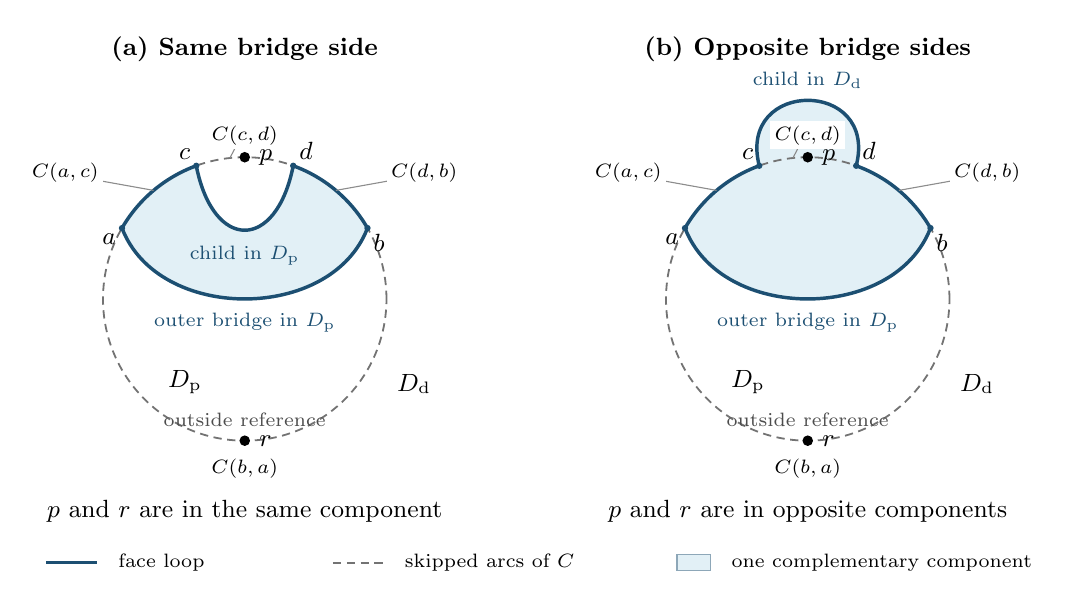
\begin{tikzpicture}[x=1cm,y=1cm,font=\small,
  tour/.style={draw=black!55,densely dashed,line width=.65pt},
  route/.style={draw=loopsideroute,line width=1.25pt},
  arcname/.style={font=\scriptsize,fill=white,inner sep=1.5pt},
  bridge/.style={font=\scriptsize,text=loopsideroute,inner sep=1pt},
  leader/.style={draw=black!45,line width=.4pt},
  testpoint/.style={circle,fill=black,inner sep=1.35pt}]

  \foreach \shift/\case in {0/0,7.15/1}{
    \begin{scope}[xshift=\shift cm]
      \coordinate (a) at (150:1.8);
      \coordinate (c) at (110:1.8);
      \coordinate (d) at (70:1.8);
      \coordinate (b) at (30:1.8);

      \ifnum\case=0
        \path[fill=loopsidefill]
          (a) arc[start angle=150,end angle=110,radius=1.8]
          .. controls (-.40,.60) and (.40,.60) .. (d)
          arc[start angle=70,end angle=30,radius=1.8]
          .. controls (1.10,-.30) and (-1.10,-.30) .. cycle;
      \else
        \path[fill=loopsidefill]
          (a) arc[start angle=150,end angle=110,radius=1.8]
          .. controls (-.90,2.80) and (.90,2.80) .. (d)
          arc[start angle=70,end angle=30,radius=1.8]
          .. controls (1.10,-.30) and (-1.10,-.30) .. cycle;
      \fi

      \draw[tour] (0,0) circle (1.8);
      \node at (-.76,-1.06) {$D_{\rm p}$};
      \node at (2.15,-1.08) {$D_{\rm d}$};

      \draw[route] (a)
        arc[start angle=150,end angle=110,radius=1.8];
      \draw[route] (d)
        arc[start angle=70,end angle=30,radius=1.8];
      \draw[route] (b)
        .. controls (1.10,-.30) and (-1.10,-.30) .. (a);
      \node[bridge] at (0,-.30) {outer bridge in $D_{\rm p}$};

      \ifnum\case=0
        \draw[route] (c)
          .. controls (-.40,.60) and (.40,.60) .. (d);
        \node[bridge] at (0,.55) {child in $D_{\rm p}$};
        \node[font=\small\bfseries] at (0,3.17)
          {(a) Same bridge side};
        \node[align=center,font=\small] at (0,-2.70)
          {$p$ and $r$ are in the same component};
      \else
        \draw[route] (c)
          .. controls (-.90,2.80) and (.90,2.80) .. (d);
        \node[bridge] at (0,2.78) {child in $D_{\rm d}$};
        \node[font=\small\bfseries] at (0,3.17)
          {(b) Opposite bridge sides};
        \node[align=center,font=\small] at (0,-2.70)
          {$p$ and $r$ are in opposite components};
      \fi

      \draw[leader] (-2.00,1.53) -- (130:1.8);
      \node[arcname] at (-2.28,1.60) {$C(a,c)$};
      \draw[leader] (2.00,1.53) -- (50:1.8);
      \node[arcname] at (2.28,1.60) {$C(d,b)$};
      \draw[leader] (-.10,1.96) -- (96:1.8);
      \node[arcname] at (0,2.08) {$C(c,d)$};
      \node[arcname] at (0,-2.16) {$C(b,a)$};

      \foreach \point/\place in {a/below left,c/above left,
                                  d/above right,b/below right}{
        \fill[loopsideroute] (\point) circle (1.15pt);
        \node[\place,inner sep=2pt] at (\point) {$\point$};
      }
      \node[testpoint,label={[inner sep=3pt]right:$p$}] at (0,1.8) {};
      \node[testpoint,label={[inner sep=3pt]right:$r$}] at (0,-1.8) {};
      \node[font=\scriptsize,text=black!70] at (0,-1.53)
        {outside reference};
    \end{scope}
  }

  \draw[route] (-2.52,-3.35) -- (-1.88,-3.35);
  \node[anchor=west,font=\scriptsize] at (-1.73,-3.35)
    {face loop};
  \draw[tour] (1.12,-3.35) -- (1.76,-3.35);
  \node[anchor=west,font=\scriptsize] at (1.91,-3.35)
    {skipped arcs of $C$};
  \path[fill=loopsidefill,draw=loopsideroute!50,line width=.4pt]
    (5.49,-3.45) rectangle (5.91,-3.25);
  \node[anchor=west,font=\scriptsize] at (6.06,-3.35)
    {one complementary component};
\end{tikzpicture}
\endgroup
